\section{Results} \label{sec:results}

This section presents the results for all tuning runs for the TSP instances of
sizes 532 and 85900.  Figures~\ref{fig:85900boxplot} and~\ref{fig:532boxplot}
show the distributions of the costs of the best solutions found for the
instance of size 85900 after 4 separate runs. It shows data for 2 and 4 virtual
machines hosted in the cloud and receiving different numbers of simultaneous
result requests.  The figure shows the distribution of the results obtained by
running the autotuner in the target machine with the unmodified OpenTuner.

\begin{figure}[htpb]
    \centering
    \begin{minipage}{.48\textwidth}
        \centering
        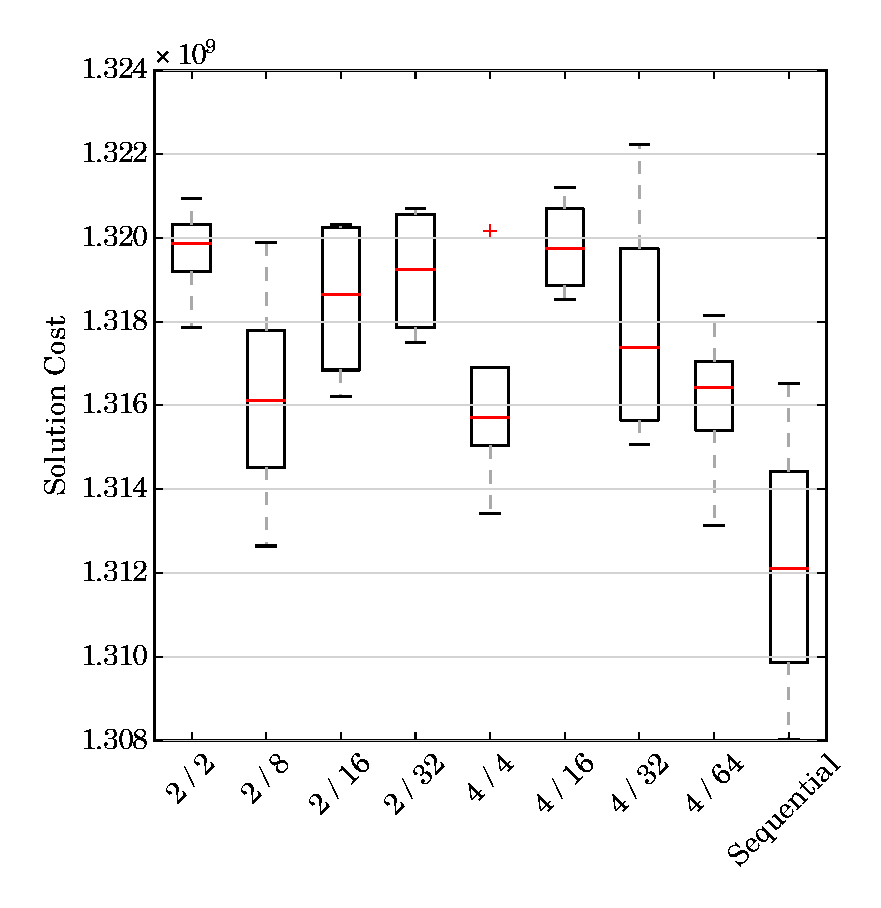
\includegraphics[scale=.48]{pla85900_15min_boxplot}
        \caption{Boxplots of 4 runs solving an instance of size 85900 with
                 different numbers of VMs and requests per VM.}
        \label{fig:85900boxplot}
    \end{minipage}%
    \hfill
    \begin{minipage}{.48\textwidth}
        \centering
        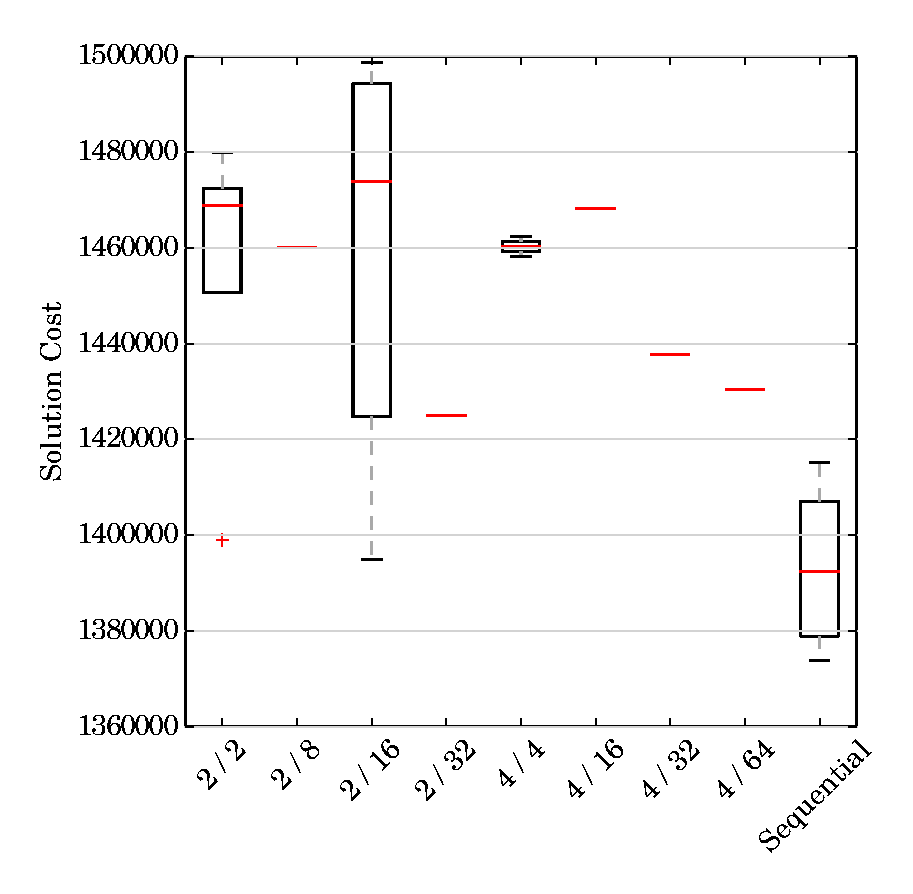
\includegraphics[scale=.48]{att532_15min_boxplot}
        \caption{Boxplots of 4 runs solving an instance of size 532 with
                 different numbers of VMs and requests per VM.}
        \label{fig:532boxplot}
    \end{minipage}%
    \label{fig:boxplots}
\end{figure}

Figures~\ref{fig:532tspi2} and~\ref{fig:532tspi4} show the best
runs in the instance of size 532 for the unmodified OpenTuner and
for each virtual machine configuration.
Figures~\ref{fig:85900tspi2} and~\ref{fig:85900tspi4} show the same
measurements for the instance of size 85900.
The time overhead in relation to the unmodified OpenTuner is clearly
visible in Figures~\ref{fig:532tspi2} to~\ref{fig:85900tspi4}, and is
due to the initialization of the cloud application.

\begin{figure}[htpb]
    \centering
    \begin{minipage}{.48\textwidth}
        \centering
        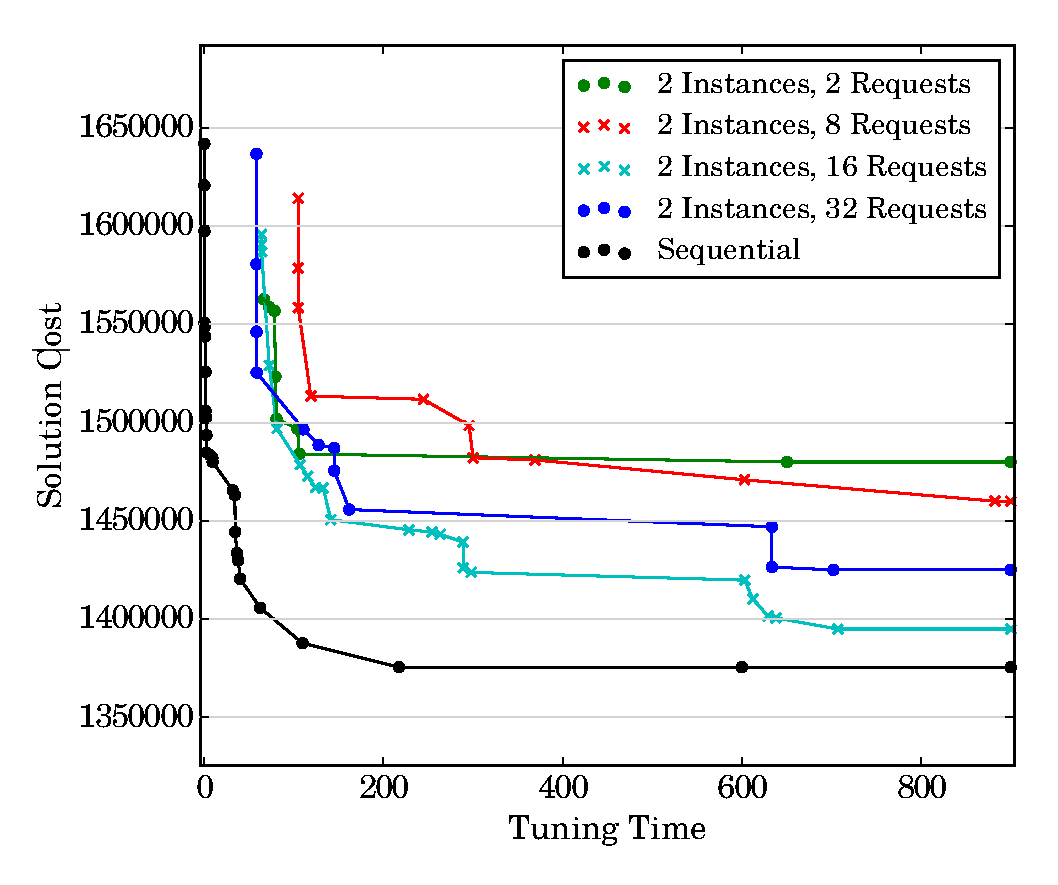
\includegraphics[scale=.43]{i2_p_n_comparison}
        \caption{Measurements using two virtual machine instances, solving
                 a TSP instance of size 532.}
        \label{fig:532tspi2}
    \end{minipage}%
    \hfill
    \begin{minipage}{.48\textwidth}
        \centering
        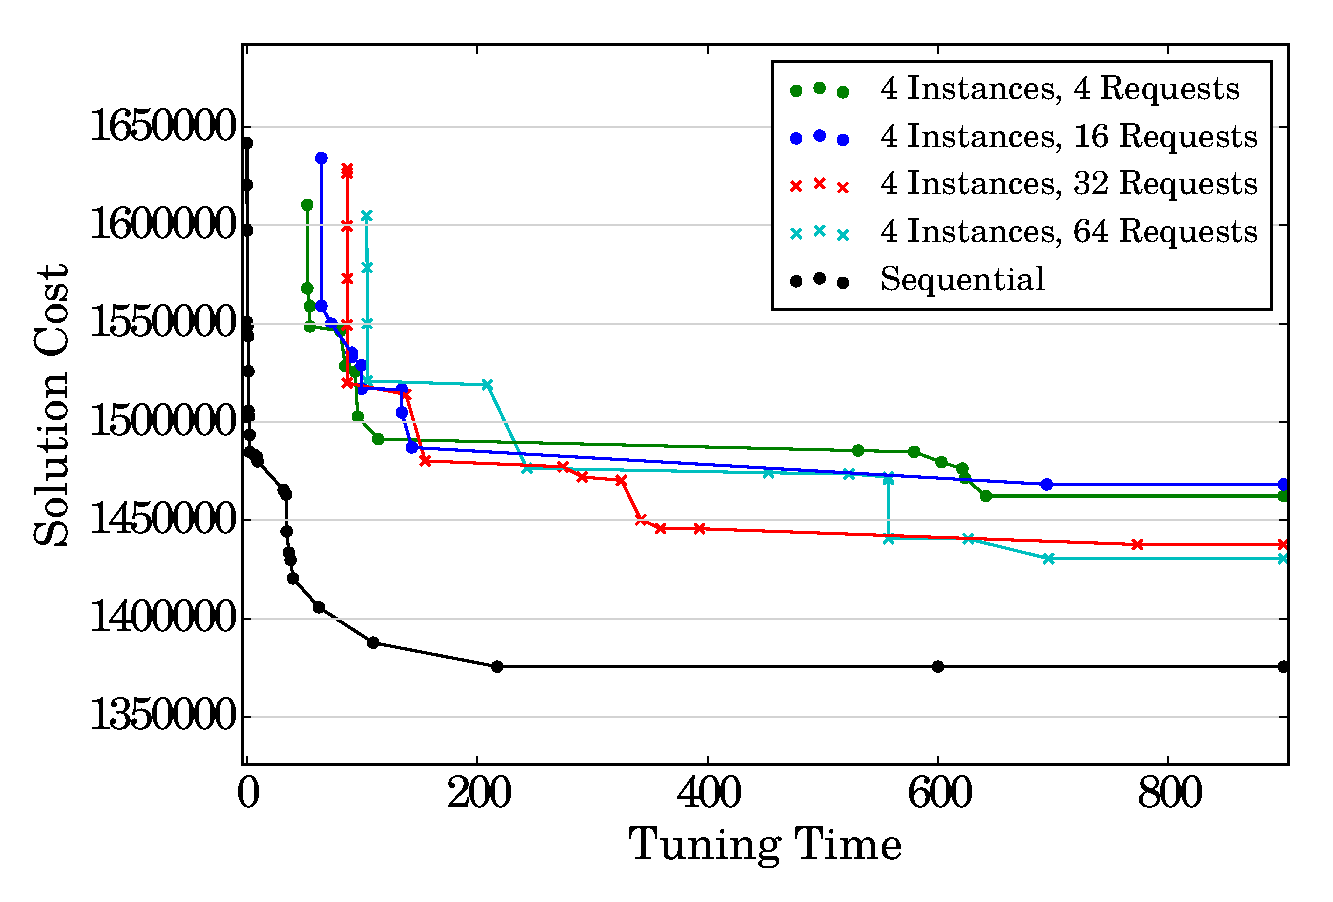
\includegraphics[scale=.43]{i4_p_n_comparison}
        \caption{Measurements using four virtual machine instances,
                 solving a TSP instance of size 532.}
        \label{fig:532tspi4}
    \end{minipage}%
    \label{fig:532tsp}
\end{figure}

The tuning runs using our methodology and protocol depend on the initialization
of a cloud application, and start to produce results later in the tuning run.
The cost of running the same virtual machine instance used in our experiments
with the Google Compute Engine were as low as
US\$0.038~\footnote{\path{cloud.google.com/compute/pricing#predefined_machine_types}
[Accessed on 23 December 2015]} per hour, per instance. The cost of obtaining
an autotuned solution of a given quality with our methodology is therefore
considerably lower than the cost of acquiring a machine capable of finding
the same solution.

\begin{figure}[htpb]
    \centering
    \begin{minipage}{.48\textwidth}
        \centering
        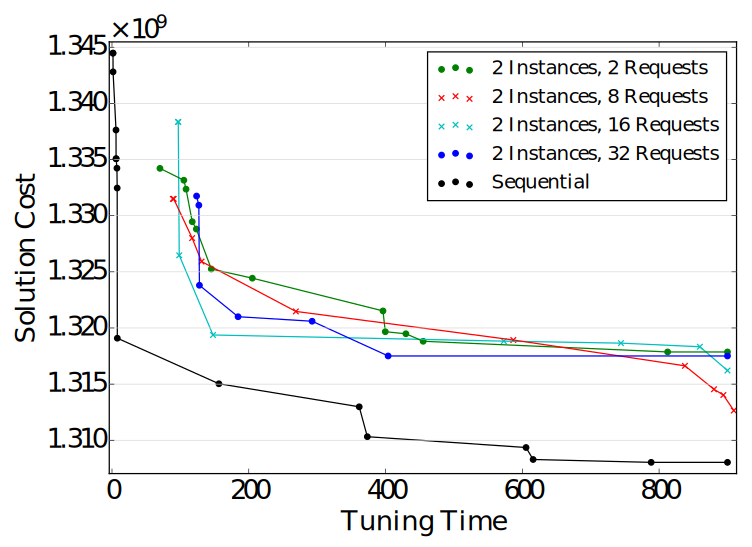
\includegraphics[scale=.43]{i2_p_n_comparison_85900}
        \caption{Measurements using two virtual machine instances,
                 solving an instance of size 85900.}
        \label{fig:85900tspi2}
    \end{minipage}%
    \hfill
    \begin{minipage}{.48\textwidth}
        \centering
        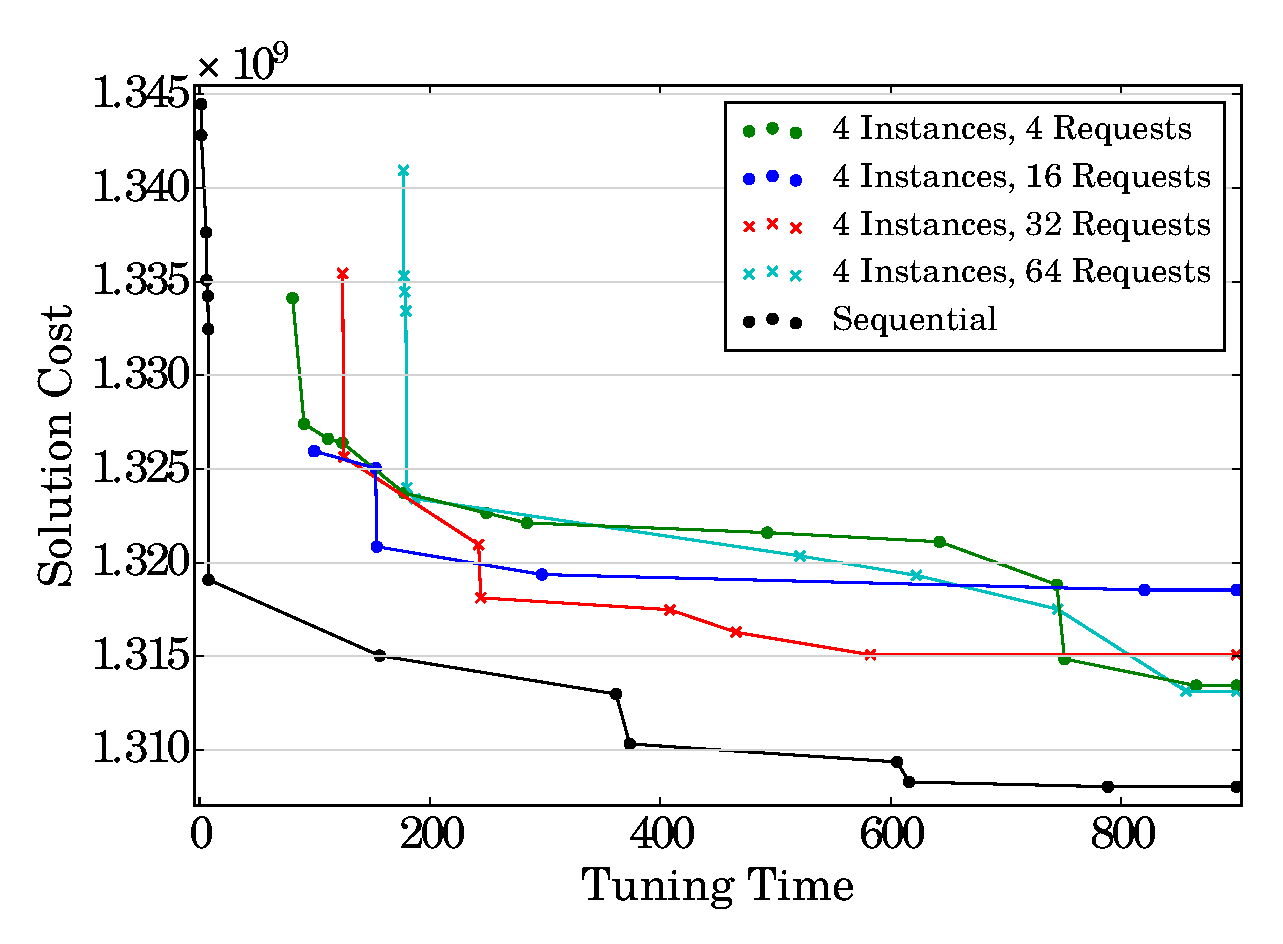
\includegraphics[scale=.43]{i4_p_n_comparison_85900}
        \caption{Measurements using four virtual machine instances,
                 solving an instance of size 85900.}
        \label{fig:85900tspi4}
    \end{minipage}%
    \label{fig:85900tsp}
\end{figure}
